\subsection{Computing the heuristic}\label{sec:computation}

We present an algorithm to efficiently compute our heuristics (pseudocode
in~\cref{sec:heuristic-code}). At a high level, we rephrase the minimization of
costs (over paths) to a maximization of \emph{scores} (over chains of matches).
We initialize the heuristic by precomputing all seeds, matches, potentials and a
\emph{contours} data structure used to compute the maximum number of matches on
a chain. During the \A~search, the heuristic is evaluated in all explored
states, and the contours are updated whenever a match gets pruned.

\paragraph{Scores} The \emph{score of a match} $m$ is
$\matchscore(m){:=}r{-}\matchcost(m)$ and is always positive. The \emph{score of
a $\preceq_p$-chain} $m_1\preceq_p \dots \preceq_p m_l$ is the sum of the scores
of the matches in the chain. We define the chain score of a match $m$ as
\begin{equation}
S_p(m):=\max_{m\preceq_p m_1\preceq_p\dots \preceq_p m_l\preceq_p v_t}\big\{\matchscore(m) + \dots + \matchscore(m_l)\big\}.
\label{eq:chain}
\end{equation}
Since $\preceq_p$ is a partial order, $S_p$ can be computed with
base case ${S_p(m_\omega) = 0}$ and the recursion
\begin{equation}
S_p(m) = \matchscore(m) + \max_{m\preceq_p m' \preceq v_t} S_p(m').
\label{eq:chainscore}
\end{equation}
We also define the chain score of a state $u$ as the maximum chain score over
succeeding matches $m$: $S_p(u) = \max_{u\preceq_p m \preceq_p v_t} S_p(m)$, so that
\cref{eq:chainscore} can be rewritten as $S_p(m) = \matchscore(m) +
S_p(\matchend(m))$.

\begin{figure}[t]
  \centering
  \subfloat[SH]{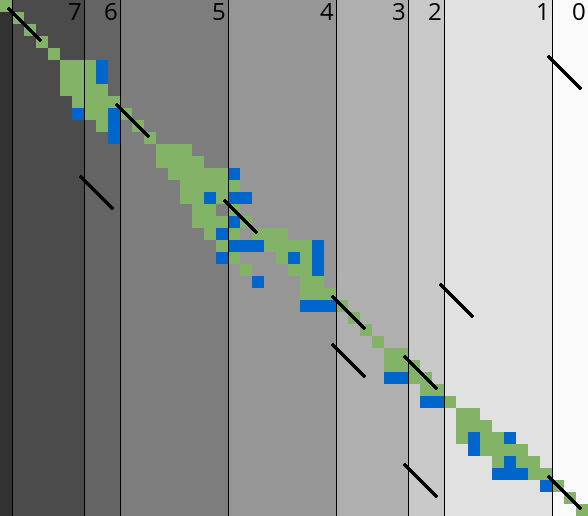
\includegraphics[width=0.32\linewidth]{imgs/layers/sh-noprune.png}\label{fig:layers-sh}}
  \hfill
  \subfloat[CSH]{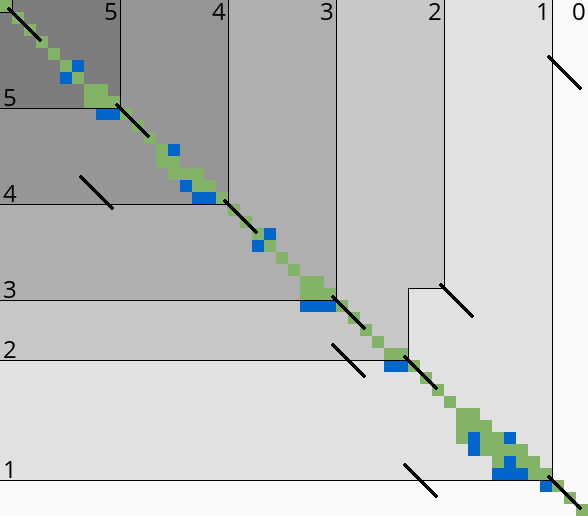
\includegraphics[width=0.32\linewidth]{imgs/layers/csh-noprune.png}\label{fig:layers-csh}}
  \hfill
  \subfloat[\GCH]{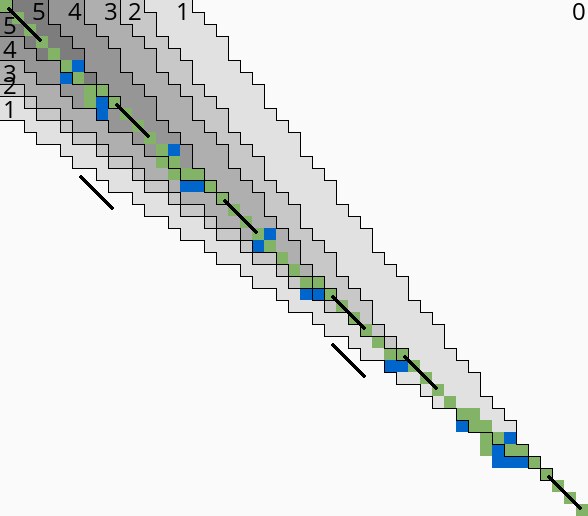
\includegraphics[width=0.32\linewidth]{imgs/layers/gcsh-noprune.png}\label{fig:layers-gcsh}}
  \\
  \subfloat[SH + pruning]{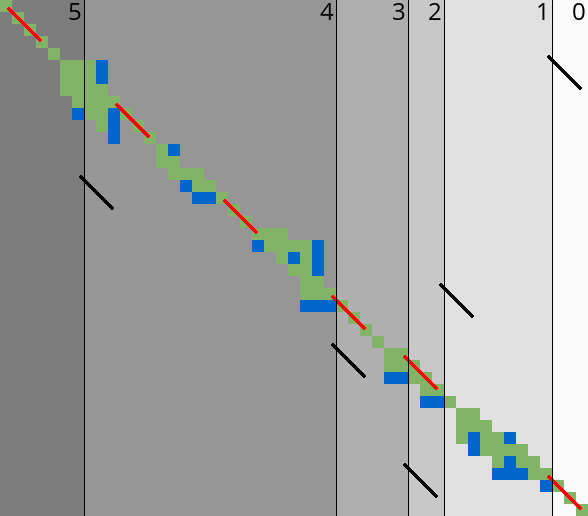
\includegraphics[width=0.32\linewidth]{imgs/layers/sh.png}\label{fig:layers-sh-pruning}}
  \hfill
  \subfloat[CSH + pruning]{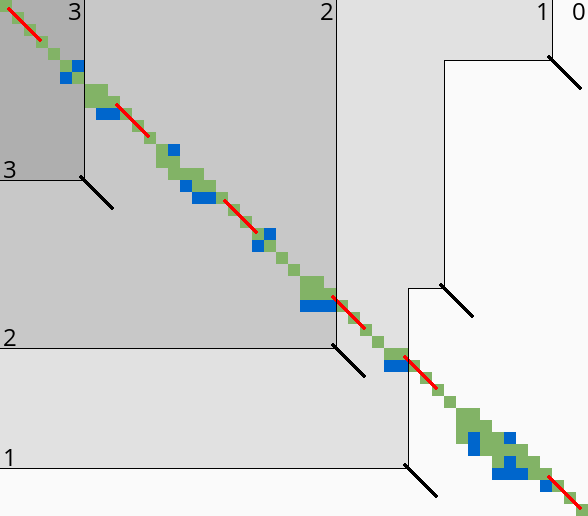
\includegraphics[width=0.32\linewidth]{imgs/layers/csh.png}\label{fig:layers-csh-pruning}}
  \hfill
  \subfloat[\GCH +
  pruning]{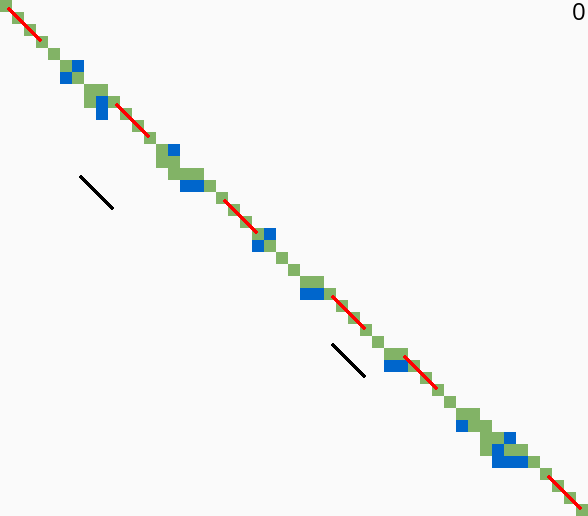
\includegraphics[width=0.32\linewidth]{imgs/layers/gcsh.png}\label{fig:layers-gcsh-pruning}}
  \caption[Contours and layers of different seed heuristics]{\textbf{Contours and layers of different heuristics after aligning}
  ($n{=}48$, $m{=}42$, $r{=}1$, $k{=}3$, edit distance $10$). Exact matches are
  black diagonal segments~(\blackmatch{}). The background colour indicates
  $S_p(u)$, the maximum number of matches on a $\preceq_p$-chain from $u$ to the
  end starting, with $S_p(u) = 0$ in white. The thin black boundaries of these
  regions are \emph{Contours}. The states of layer $\layer_\ell$ \emph{precede}
  contour $\ell$. Expanded states are green~(\greensquare{}), open states
  blue~(\bluesquare{}), and pruned matches red~(\redmatch{}). Pruning matches
  changes the contours and layers. \GCH ignores matches $m{\npreceq_T}v_t$.}
  \label{fig:contours}
\end{figure}


The following theorem allows us to rephrase the heuristic in terms of
potentials and scores for heuristics that use $\gamma {=} \seedcost$ and respect
the order of the seeds, which is the case for $\hsh$ and $\hcsh$ (proof
in~\cref{app:computation}):
\begin{restatable}{thm}{thmcomputation}\label{lem:computation}
$h^\matches_{p,\seedcost}(u) = P(u) - S_p(u)$ for any partial order~$\preceq_p$
that is a refinement of $\preceq_i$ (i.e. $u\preceq_p v$ must imply $u\preceq_i
v$).
\end{restatable}

\paragraph{Layers and contours}
We compute $\hsh$ and $\hcsh$ efficiently using \emph{contours}. Let
\emph{layer} $\layer_\ell$ be the set of states $u$ with score $S_p(u) \geq
\ell$, so that $\layer_\ell \subseteq \layer_{\ell{-}1}$. The $\ell$th
\emph{contour} is the boundary of $\layer_\ell$~(\cref{fig:contours}).
Layer~$\layer_\ell$~($\ell>0$) contains exactly those states that precede a
match $m$ with score $\ell \leq S_p(m) < \ell+r$ (\cref{lem:contour} in
\cref{app:computation}).

\paragraph{Computing $S_p(u)$}
This last observation inspires our algorithm for computing chain scores. For
each layer $\layer_\ell$, we store the set
$L[i]$~of matches having score $\ell$: ${L[\ell] = \{m\in \matches \mid S_p(m) =
\ell\}}$.
%
The score $S_p(u)$ is then the highest~$\ell$ such that
layer $L[\ell]$ contains a match $m$ reachable from $u$ ($u\preceq_p m$).
%
From~\cref{lem:contour} we know that $S_p(u) \geq \ell$ if and only if one of
the layers $L[\ell']$ for $\ell'\in [\ell, \ell+r)$ contains a match preceded
by $u$. We use this to compute $S_p(u)$ using a binary search over the layers $\ell$.
%
We initialize $L[0] {=} \{m_{\omega}\}$ ($m_{\omega}$ is a fictive match at the
target $v_t$), sort all matches in $\matches$ by~$\preceq_p$, and process them in
decreasing order (from the target to the start). After computing
$S_p(\matchend(m))$, we add~$m$ to layer $S_p(m) = \matchscore(m) +
S_p(\matchend(m))$. Matches that do not precede the target ($\matchstart(m) \not
\preceq_p m_\omega$) are ignored.

\paragraph{Pruning matches from $L$}
When pruning matches starting or ending in state~$u$ in layer $\ell_u=S_p(u)$,
we remove all matches that start at $u$ from layers $L[\ell_u{-}r{+}1]$ to
$L[\ell_u]$, and all matches starting in some~$v$ and ending in~$u$ from layers
$L[\ell_v{-}r{+}1]$ to $L[\ell_v]$.

Pruning a match may change $S_p$ in layers above~$\ell_u$, so we update them
after each prune. We iterate over increasing $\ell$ starting at
$\ell_u+1$ and recompute ${\ell':=S_p(m)\leq \ell}$ for all matches $m$ in
$L[\ell]$. If $\ell' \neq \ell$, we move $m$ from $L[\ell]$ to $L[\ell']$. We
stop iterating when either $r$ consecutive layers were left
unchanged, or when all matches in $r-1+\ell-\ell'$ consecutive layers have
shifted down by the same amount $\ell-\ell'$. In the former case, no further
scores can change, and in the latter case, $S_p$ decreases by $\ell-\ell'$
for all matches with score $\geq \ell$. We remove the emptied layers
${L[\ell'+1]}$ to $L[\ell]$ so that all higher layers shift down by
$\ell-\ell'$.

\paragraph{\SH} Due to the simple structure of the \sh, we also simplify its
computation by only storing the start of each layer and the number of matches in
each layer, as opposed to the full set of matches.

\paragraph{\GCH}
\Cref{lem:computation} does not apply to \gch since it uses chaining cost
$\gamma{=}\max(\gapcost(u, v), \seedcost(u,v))$ which is different from
$\seedcost(u,v)$. It turns out that in this new setting it is never optimal to chain
two matches if the gap cost between them is higher than the seed cost.
Intuitively, it is better to miss a match than to incur additional gapcost to
include it. We capture this constraint by introducing a transformation $T$ such
that $u\preceq_T v$ holds if and only if $\seedcost(u,v) \geq \gapcost(u,v)$, as
shown in~\cref{app:gapcost-proof}. Using an additional \emph{consistency}
constraint on the set of matches we can compute $\hgchM$ via $S_T$ as before.

\begin{definition}[Consistent matches]\label{dfn:consistent} %
  A set of matches $\matches$ is \emph{consistent} when for each $m\in\matches$
  (from $\st ij$ to $\st {i'}{j'}$) with $\matchscore(m) {>} 1$, for each
  \emph{adjacent} pair of existing states $(\st i{j{\pm}1}, \st{i'}{j'})$ and
  $(\st ij, \st {i'}{j'{\pm}1})$, there is an \emph{adjacent} match with corresponding start and
  end, and score at least $\matchscore(m){-}1$.
\end{definition}
This condition means that for $r{=}2$, each exact match must be adjacent to four
(or less around the edges of the graph) inexact matches starting or ending in
the same state. Since we find all matches $m$ with $\matchcost(m){<}r$, our initial set
of matches is consistent. To preserve consistency, we do not prune matches if
that would break the consistency of $\matches$.

\begin{restatable}[Gap transformation]{definition}{transformation}\label{dfn:transformation} %
  The partial order $\preceq_T$ on states is induced by comparing both
  coordinates after the \emph{gap transformation}
% Numbered because it may be referred externally.
\begin{equation*}
  T: \quad\st{i}{j}\mapsto \tst{i - j - P\st{i}{j}}{j-i-P\st{i}{j}}
\end{equation*}
\end{restatable}

\begin{restatable}{thm}{thmgapcost}\label{lem:gapcost}%
 Given a \emph{consistent} set of matches $\matches$, the \gch can be computed
 using scores in the transformed domain:
\begin{equation*}
  \hgchM(u) =
  \begin{cases}
    \Pot(u) - S_T(u) & \text{if $u\preceq_T v_t$,} \\
    \gapcost(u, v_t) & \text{if $u\npreceq_T v_t$.}
  \end{cases}
\end{equation*}
\end{restatable}

\paragraph{Asymptotic scaling}
Using the transformation of the match coordinates, we can now reduce $\gscost$
to $\seedcost$ and efficiently compute \GCH in any explored state. The worst
case preprocessing time is $\Oh(n+r\log r)$ and the worst case query of the
heuristic is $\Oh(\log^2 r) = \Oh(\log^2 n)$ when implemented with binary search
to find a layer and a search tree within each layer. In practice, optimizations
for the empirical runtime bring the worst case for querying to potentially
looking up each match: $\Oh(r) = \Oh(n^2)$.
